\documentclass[..thesis.tex]{subfiles}

\usetikzlibrary{3d}
\usetikzlibrary{patterns}

\tikzset{xyp/.style={canvas is xy plane at z=#1}}
\tikzset{xzp/.style={canvas is xz plane at y=#1}}
\tikzset{yzp/.style={canvas is yz plane at x=#1}}


\begin{document}

\toguide{Okay, what's next?}

The key challenge for Goblint is the number of false-positives. It is clear that even if one can guarantee the soundness of the 
underlying analysis, then there is a threshold of incorrect warnings above what the results of the analysis contain too much noice
to be of help for a programmer.

\toguide{I buy it, what can be done about it?}

One of the steps taken to reduce the the number of false-positives is the usage of \textit{happen-before} relation.

\toguide{How can you use happen-before here?}

Consider following device driver:

\begin{lstlisting}[language=c,style=def]

static int i = 0;
static int j = 0;

static int file_open(file f, ...)
{
    printk( "Opening device \n");
    j += 1;
    return 0;
}

static int file_open(file f, ...)
{
    printk( "Opening device \n");
    j -= 1;
    return 0;
}

struct file_operations f_ops = {
  .open    = file_open,
  .release = file_close,
};

int init(...)
{
  publish_file_operations(f_ops);
  i += 1;
  return 0;
}

int exit(...)
{
  i -= 1;
  return 0;
}

\end{lstlisting}

As mentioned previously, \textit{init} and \textit{exit} functions are used by kernel register and de-register a device. As after publishing the file operations, Goblint cannot assume that the functions of the driver are called by one thread, a possible data-race is detected between the operations on variable $i$ in functions \textit{init} and \textit{exit}. At same time, the Linux Kernel does not allow a call to the \textit{exit} function until the call to the \textit{init} function is called and all the opened files are released.

We would like to have Goblin know about that guarantee and make use of the information that the call to \textit{init} will always complete before call to \textit{exit}.

\toguide{Example makes sense, but how to practically make use of it?}

To do so, we extend the region based analysis of Goblint.

\toguide{Erghh, was not the easiest part of the Goblint section. A bit of refreshment would be great.}

As discussed in previous section, Goblint tries to track the memory regions of pointers and uses this information to exclude possible data races.

\toadd{Region analyses covred in Goblint section.} 

For example, let us have two procedures , $f$ and $g$ that can be ran simoultanously in different threads.

\begin{lstlisting}[language=c,style=def]

int* p;
int* q;

void f()
{
  &p = &q - 1; 
}

void g()
{
  &q = &q + 1; 
}

\end{lstlisting}

 

 If we can divide the memory used by the program to two regions, $A$ and $B$ that are disjoint and we can guarantee that the pointer $p$ points to integer variable stored in region $A$ and $q$ points to integer variable stored in region $B$ then we can safely assume that there can be no data-race between the increment and decrement operations in function $f$ and $g$.

\begin{figure}[H]
  \centering
    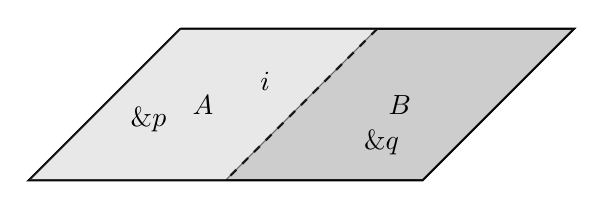
\begin{tikzpicture}
      \pgfmathsetmacro{\cubex}{5}
      \pgfmathsetmacro{\cubey}{5}
      \pgfmathsetmacro{\cubez}{5}
      \draw[thick,-] (0,0,0) -- ++(\cubex,0,0) -- ++(0,0,\cubez) -- ++(-\cubex,0,0) --  ++(0,0,-\cubez);
      \draw[thick,dashed] (0.5*\cubex,0,0) -- ++(0,0,\cubez);
      \fill[opacity=0.3,black!30,draw=black,xzp=0] (0,0) rectangle (2.5,5);
      \fill[opacity=0.3,black!65,,draw=black,xzp=0] (2.5,0) rectangle (5,5);
      \node at (0.25*\cubex,0,2.5) (A) {$A$};
      \node at (0.75*\cubex,0,2.5) (B) {$B$};

      \node at (0.15*\cubex,0,0.6*\cubez) (p) {$\&p$};
      \node at (0.8*\cubex,0,0.75*\cubez) (q) {$\&q$};

      \node at (0.35*\cubex,0,0.35*\cubez) (q) {$i$};
    \end{tikzpicture}
    \caption{Memory partition as done by region analyses}
\end{figure}

Going back to the example driver, this does allow to eliminate the data race between the assignments to $i$ in $init$ and $exit$ functions. However, if we would enhance the region analyses with one more dimension that would roughly correspond to time, we could divide the memory as seen on the following illustration. 

\begin{figure}[H]
  \centering
    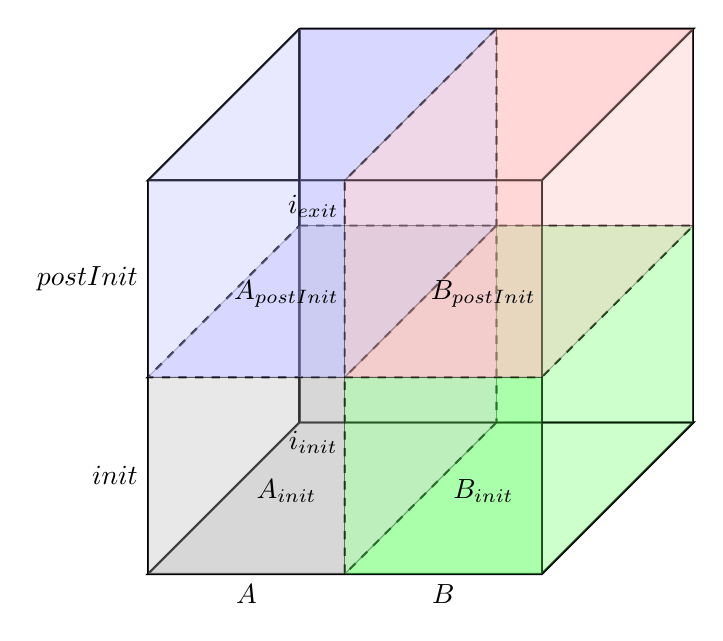
\begin{tikzpicture}
      \pgfmathsetmacro{\cubex}{5}
      \pgfmathsetmacro{\cubey}{5}
      \pgfmathsetmacro{\cubez}{5}
      \draw[thick,-] (0,0,0) -- ++(\cubex,0,0) -- ++(0,0,\cubez) -- node [anchor = north] {$B$} ++(-0.5*\cubex,0,0) --  node [anchor = north] {$A$} ++(-0.5*\cubex,0,0)  --   ++(0,0,-\cubez);
      \draw[thick,-] (0,\cubey,0) -- ++(\cubex,0,0) -- ++(0,0,\cubez) -- ++(-\cubex,0,0) --   ++(0,0,-\cubez)  ;
      \draw[thick,dashed] (0,0.5*\cubey,0) -- ++(\cubex,0,0) -- ++(0,0,\cubez) -- ++(-\cubex,0,0) --  ++(0,0,-\cubez);
      \draw[thick,-] (0,0,0) -- (0,\cubey,0);
      \draw[thick,-] (\cubex,0,0) -- (\cubex,\cubey,0);
      \draw[thick,-] (0,0,\cubez) -- node[anchor= east] {$init$} ++(0,0.5*\cubey,0)  -- node[anchor= east] {$postInit$}  ++(0,0.5*\cubey,0);
      \draw[thick,-] (\cubex,0,\cubez) -- ++(0,\cubey,0);

      
      
      \draw[thick,dashed] (0.5*\cubex,0,0) -- ++(0,0,\cubez) -- ++(0,\cubey,0) -- ++(0,0,-\cubez) -- ++(0,-\cubey,0);
      \draw[thick,dashed] (0.5*\cubex,0.5*\cubey,0) -- ++(0,0,\cubez); 

      \fill[opacity=0.3,black!30,draw=black,xzp=0] (0,0) rectangle (0.5*\cubex,\cubez);
      \fill[opacity=0.3,black!30,draw=black,xyp=0] (0,0) rectangle (0.5*\cubex,0.5*\cubey);
      \fill[opacity=0.3,black!30,draw=black,xyp=\cubez] (0,0) rectangle (0.5*\cubex,0.5*\cubey);

      \fill[opacity=0.3,blue!30,draw=black,xzp=\cubez] (0,0) rectangle (2.5,5);
      \fill[opacity=0.3,blue!30,draw=black,xzp=0.5*\cubez] (0,0) rectangle (2.5,5);
      \fill[opacity=0.3,blue!30,draw=black,xyp=0] (0,0.5*\cubey) rectangle ++(0.5*\cubex,0.5*\cubey);
      \fill[opacity=0.3,blue!30,draw=black,xyp=\cubez] (0,0.5*\cubey) rectangle ++(0.5*\cubex,0.5*\cubey);

      \fill[opacity=0.3,green!65,draw=black,xzp=0] (2.5,0) rectangle (\cubex,\cubez);
      \fill[opacity=0.3,green!65,draw=black,xyp=0] (0.5*\cubex,0) rectangle ++(0.5*\cubex,0.5*\cubey);
      \fill[opacity=0.3,green!65,draw=black,xyp=\cubez] (0.5*\cubex,0) rectangle ++(0.5*\cubex,0.5*\cubey);

      \fill[opacity=0.3,red!30,draw=black,xzp=\cubey] (2.5,0) rectangle (\cubex,\cubez);
      \fill[opacity=0.3,red!30,draw=black,xzp=0.5*\cubey] (2.5,0) rectangle (\cubex,\cubez);
      \fill[opacity=0.3,red!30,draw=black,xyp=0] (0.5*\cubex,0.5*\cubey) rectangle ++(0.5*\cubex,0.5*\cubey);
      \fill[opacity=0.3,red!30,draw=black,xyp=\cubez] (0.5*\cubex,0.5*\cubey) rectangle ++(0.5*\cubex,0.5*\cubey);


      \node at (0.265*\cubex,0.125*\cubey,0.775*\cubez) (A) {$A_{init}$};
      \node at (0.765*\cubex,0.125*\cubey,0.775*\cubez) (B) {$B_{init}$};
      \node at (0.265*\cubex,0.625*\cubey,0.775*\cubez) (Ap) {$A_{postInit}$};
      \node at (0.765*\cubex,0.625*\cubey,0.775*\cubez) (Bp) {$B_{postInit}$};

      
      \node at (0.285*\cubex,0.2*\cubey,0.65*\cubez) (ip) {$i_{init}$};
      \node at (0.285*\cubex,0.8*\cubey,0.65*\cubez) (i) {$i_{exit}$};
    \end{tikzpicture}
    \caption{Memory partition with addition of time dimension}
\end{figure}

This would let Goblint exclude the possibilty of race between these two opretations. 

\toguide{How is it done?}
1
To do this, Goblint needs to track information for each read and write operation.

\toask{operation bad word?}

The information tracked is divided into \textit{left} and \textit{right} side. 

On the left side, information regarding the memory region of the variable is stored as a set of sets, $C$, such that every element of $C$, $I$ describes an intersection of memory regions.

In our example driver, the $C$ for the increment operation in the $init$ function would be 

\begin{equation*}
\lb \lb A, init \rb \rb \text{.}
\end{equation*} 

On the right side, information regarding possible reasons why data race cannot take place with another read or write operation is stored in a set $M$. For an example, $M$ could contain the set of locks held at the specific operation or wether or not the thread running the procedure containing the operation is guaranteed to be unique.

When deciding if there is a possibility of a data race between operations $a$ and $b$, Goblint uses two predicates, $L$ and $R$ to evaluate left and right sides of these operations. 

The first of those predicates is defined as follows

\begin{equation*}
L \lp C_a, C_b \rp = \left| C_a \cap C_b \right| > 0 \text{.}
\end{equation*}

If $L \lp C_a, C_b \rp$ evaluates to false it means that the two operations do not share a common memory region and hence there cannot be a data race. 

The second predicate, $R$ evaluates the sets $M_a$ and $M_b$ and returns true if there is something that guarantees that the operations $a$ and $b$ cannot race. For example, it could be when performing both of these operations, lock $l$ must be held or in case of $a=b$, there is a guarantee that there can be only one thread running that executes the operation.

Equipped with those definitions, we can guarantee that operations $a$ and $b$ cannot race if the implication

\begin{equation}
\label{implication}
L \lp C_a, C_b \rp \implies R \lp M_a, M_b \rp  
\end{equation}

holds.

Comming back to our example driver, one can see that using the enhanced region analyses, we can now see that there cannot be a race between $i_{init}$ and $i_{exit}$. Indeed, as

\begin{equation*}
 \lb \lb A, init \rb \rb \cap  \lb \lb A, postInit \rb \rb = \emptyset
\end{equation*}

then $L \lp C_{i_{init}}, C_{i_{postInit}} \rp$ is false and the implication (\ref{implication}) holds for $i_{init}$ and $i_{exit}$.

As an example of right hand sides excuding an data race, if we take both $a$ and $b$ to be $i_{init}$ then when evaluating 

\begin{equation*}
R \lp M_{i_{init}}, M_{i_{init}} \rp
\end{equation*} 

we can take into account that Linux kernel does not allow one to register the same driver more than once and as such, we can guarantee that the thread running the $init$ function is unique.

Based on that information $R \lp M_{i_{init}}, M_{i_{init}} \rp$ holds and so does the implication (\ref{implication}).



\end{document}